\documentclass{amsart}
\usepackage{amsaddr}
\usepackage{amssymb}
\usepackage[latin1]{inputenc}
\usepackage[swedish,english]{babel}
\usepackage{ifpdf}
\ifpdf
\usepackage[pdftex]{graphicx}
\usepackage{epstopdf}
\else
\usepackage[dvips]{graphicx}
\fi
% \usepackage{subfigure}
% \usepackage{sidecap}
\usepackage[pdftitle={Robin Eriksson - H1},
pdfauthor={Robin Eriksson},
pdffitwindow=true,
breaklinks=true,
colorlinks=true,
urlcolor=blue,
linkcolor=red,
citecolor=red,
anchorcolor=red]{hyperref}
% \usepackage{pdfpages}
\usepackage{algorithm}
% \usepackage{algorithmic}
\usepackage[noend]{algpseudocode}
\usepackage{dsfont}
\usepackage[numbers,sort&compress]{natbib}
\usepackage{appendix}
\usepackage[section]{placeins}
% **************************************************************************
\usepackage[margin=1.25in]{geometry}
\usepackage{subcaption}
% ***************************************************************************
\usepackage{microtype}
\usepackage{parskip}

\usepackage{listings}
\usepackage{color} %red, green, blue, yellow, cyan, magenta, black, white
\definecolor{mygreen}{RGB}{28,172,0} % color values Red, Green, Blue
\definecolor{mylilas}{RGB}{170,55,241}
% ***************************************************************************
\numberwithin{equation}{section}
\numberwithin{table}{section}
\numberwithin{figure}{section}

\theoremstyle{plain}
\newtheorem{theorem}{Theorem}[section]
\newtheorem{lemma}[theorem]{Lemma}
\newtheorem{proposition}[theorem]{Proposition}
\newtheorem{corollary}[theorem]{Corollary}
\newtheorem{conjecture}[theorem]{Conjecture}
% \newtheorem{algorithm}[theorem]{Algorithm}
% \newtheorem{criterion}[theorem]{Criterion}

\theoremstyle{definition}
\newtheorem{definition}{Definition}[section]
\newtheorem{assumption}[definition]{Assumption}
\newtheorem{convention}[definition]{Convention}
\newtheorem{example}[definition]{Example}
% \newtheorem{problem}[definition]{Problem}

\theoremstyle{remark}
\newtheorem*{remark}{Remark}
% \newtheorem*{note}{Note}
% \newtheorem*{notation}{Notation}
% \newtheorem*{summary}{Summary}
% \newtheorem{theorem}{Theorem}[section]
% \newtheorem{lemma}[theorem]{Lemma}

\renewcommand{\Pr}{\mathbf{P}}
\renewcommand{\P}{P}
\newcommand{\E}{\mathbf{E}}
\newcommand{\V}{\mathbf{V}}
\newcommand{\R}{\mathbb{R}}
\newcommand{\F}{\mathcal{F}}

% *** use these commands to write comments; they are easy to spot in the text!
\newcommand{\comment}[1]{\textcolor{blue}{\{#1\}}}
\newcommand{\margincomment}[1]{* \marginpar{\textcolor{blue}{*\{#1\}}}}


% *** todo list! ***
\usepackage{enumitem,amssymb}
\newlist{todolist}{itemize}{2}
\setlist[todolist]{label=$\square$}
\usepackage{pifont}
\newcommand{\cmark}{\ding{51}}%
\newcommand{\xmark}{\ding{55}}%
\newcommand{\done}{\rlap{$\square$}{\raisebox{2pt}{\large\hspace{1pt}\cmark}}%
  \hspace{-2.5pt}}
\newcommand{\wontfix}{\rlap{$\square$}{\large\hspace{1pt}\xmark}}



% **************************************************************************

\begin{document}

\title[]{Homework 1}

\author[R. Eriksson]{Robin Eriksson}
\email{\href{mailto:robin.eriksson@it.uu.se}{robin.eriksson@it.uu.se}}
% \address{Division of Scientific Computing \\
% Department of Information Technology \\
% Uppsala University \\
% SE-751 05 Uppsala, Sweden.}

% \subjclass[2010]{Primary: NNXMM; Secondary: NNXMM}

% \keywords{}

\date{\today}


\selectlanguage{english}
%\maketitle
\section{Double-descent in random Feature regression}
The result from using random Fourier features and the minimum-norm
solution for regression on the Boston house price data
set\footnote{can be retrieved from here:
  \url{http://lib.stat.cmu.edu/datasets/boston}}. The experiment
result, see Figure~\ref{fig:double}, shows what is known as the double
descent phenomena~\cite{belkin2019reconciling}.

The experiment included testing different kernel widths, $\gamma$
values, $[0.001, 0.01, 0.1, 1]$. Interesting is that the smallest
$\gamma$ used, $0.001$ gave the quickest descent in the training error
and includes a (potential) global minima in the underparameterized
regime. However, this seems to come at the price of the $||\theta||$
as it seems strictly larger than the other $\gamma$ values tested.

\begin{figure}[h]
  \centering
  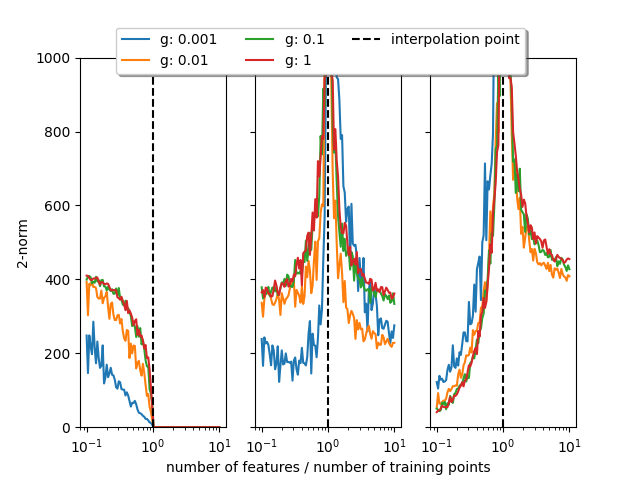
\includegraphics[width=0.9\linewidth, angle=0]{../Figure_1} %11.4 cm wide
  \caption{(left) training error (2-norm). (middle) testing error
    (2-norm). (right) $\theta$ norm. The colors represent the
    different $\gamma$ values (g for short). The dashed line is the
    interpolation point. Training and test error is the 2-norm of the
    difference between estimated and true value.}
  \label{fig:double}
\end{figure}

\bibliographystyle{plain}
\bibliography{report1}

\end{document}
